\section{Rød-svarte trær} \label{rb_tre}
Vanlige binære søketrær blir fort veldig ubalanserte. Prøv å sett inn 1, 2, 3, 4, 5, 6, 7, ... (i den rekkefølgen) i et binært søketre. Da vil vi i praksis ha en lenket liste. Da er også kjøretiden for å søke, sette inn og slette i verste fall $ O(n) $, i stedet for $ O(\log n) $ som er det vi vanligvis har for søketrær, og som er det vi ønsker. Vi trenger derfor trær som vil balansere seg selv. Vi skal se på rød-svarte trær, men det finnes også andre typer (som AVL-trær)

Rødsvarte trær er binære søketrær med noen spesielle strukturkrav. Kravene er designet for å motkjempe skjevhet (som illustrert i figur \ref{fig:bintre}), og dermed forbedre kjøretid.

Vi deler nodene opp i to kategorier, røde og svarte. Vi følger noen bestemte regler på hvordan vi skal farge nodene, og fargen på nodene avgjør som vi må benytte oss av rotasjon eller ikke (se \ref{trerotasjon}). 

\begin{definition}
	Et rød-svart tre er et binært søketre med noen spesielle tilleggsregler:
	\begin{enumerate}[i]
		\item Roten er svart.
		\item Hvis en node er rød, må barna være svarte.
		\item Enhver vei fra en node til en null-peker må inneholde samme antall svarte noder.
	\end{enumerate}
\end{definition}

Fargen til en node er ikke statisk, den kan endre seg. Disse reglene sikrer at høyden maksimalt er $ 2\log_2 (n+1) $ (bevis for dette finnes på Wikipedia).

\subsection{Insetting}
Vi zoomer inn på en del av treet og jobber kun med de nodene som har noe å si for innsetting. X er noden vi skal sette inn, P er foreldernoden, U er onkelnoden (søsken av forelder), G er besteforeldernoden. Når vi setter inn ei node i et rød-svart tre er den nye noda alltid rød. Deretter må vi se på fargene til P, U og G for å finne ut om vi må ta noen videre steg:

\begin{figure}[htb]
	\caption{Situasjon for innsetting}
	\centering
	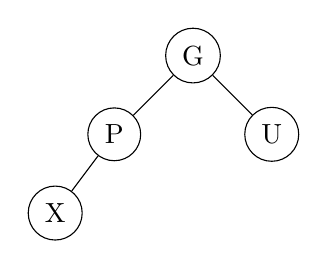
\begin{tikzpicture}[level distance=1cm,
	level 1/.style={sibling distance=2cm},
	level 2/.style={sibling distance=1.5cm},
	level 3/.style={sibling distance=1cm},
	every node/.style = {shape=circle, draw, align=center}]
	
	\node{G}
	child {node {P}
		child {node {X}}
		child [missing]{}
	}
	child {node {U}};
	\end{tikzpicture}
\end{figure}

\begin{theorem} Innsetting i rød-svarte trær
	
	\begin{itemize}
		\item Hvis P er svart er alt OK, og vi er ferdig
		\item Hvis P er rød må vi ta noen steg for å opprettholde krav \textit{ii} og \textit{iii}:
		\begin{itemize}
			\item Hvis U også er rød: Farg P og U svarte og farg G rød. Dette kan føre til trøbbel videre oppover i treet, så vi må fortsette oppover å rette opp feil.
			\item Hvis U er svart, utfør en Zig-rotasjon mhp P, og utfør nødvendige fargeendringer
		\end{itemize}
		\item Hvis rota på noe tidspunkt blir farget rød kan man bare farge den svart igjen.
	\end{itemize}
\end{theorem}


\subsection{Sletting}
Sletting fra rød-svarte trær handler til syvende og sist om å slette løvnoder. Skal vi slette en indre node kan vi gå en plass til høyre, og deretter gå til venstre helt til vi er i bunnen av treet, og swappe de to nodene. Deretter kan vi slette (det som nå er) løvnoden. Når vi gjør dette kan det hende vi bryter med noen av kravene i definisjon \ref{def:rb_tree}. Vi må derfor bruke samme type strategi som for innsetting for å rette opp feil. 

Sletting er noe mer komplisert enn innsetting. Se seksjon 12.2.3 i læreboka for gjennomgang av en del situasjoner med figurer og forklaringer. 


\subsection{Tidsanalyse}
Siden høyden til et rød-svart tre maksimalt er $ 2\log_2 (n+1) $ har vi worst case tid $ O(\log_2 n) $. Selv om vi risikerer å måtte gjøre rotasjoner er innsetningstiden også $ O(\log_2 n) $.